\input{configuration}

\title{Lecture 33 --- More Advanced Queueing Theory}

\author{Jeff Zarnett\\ \small \texttt{jzarnett@uwaterloo.ca}}
\institute{Department of Electrical and Computer Engineering \\
  University of Waterloo}
\date{\today}


\begin{document}

\begin{frame}
  \titlepage

 \end{frame}


\begin{frame}
\frametitle{New Considerations}

New considerations---or complications---arise.

We'll talk about two settings, one that I love and one that I hate: food halls and Service Ontario. 
 
No points for guessing which is which.

\end{frame}


\begin{frame}
\frametitle{Multiple Services}

At Service Ontario, every staff member can help you with any task.

But at the food hall, the Gelato place cannot provide tacos.

Are tacos and gelato interchangeable? Maybe...

\begin{center}
	\includegraphics[width=0.4\textwidth]{images/tacos.jpg}
\end{center}

\end{frame}



\begin{frame}
\frametitle{Maintenance, Planned and Unplanned}

Services have downtime, both planned and unplanned.

If the pizza oven breaks, no more pizza today.

Usually we do not think about unplanned downtime in service capacity design.


\end{frame}


\begin{frame}
\frametitle{New Things Too?}

New services can appear: what if a Banh Mi place opens?

\begin{center}
	\includegraphics[width=0.5\textwidth]{images/banh-mi.jpg}
\end{center}

Restaurant opening is rarely a surprise...


\end{frame}

\begin{frame}
\frametitle{Interchangeability}

Interchangeability of services is a spectrum:

\begin{itemize}
	\item Full; Starving? Tacos, pizza, shawarma? Just feed me now! \vspace{5em}
	\item Partial; Just a bit hungry? Want tacos, would have shawarma. \vspace{5em}
	\item None; I came for tacos and want nothing else.
\end{itemize}


\end{frame}


\begin{frame}
\frametitle{Nutritionist}

All the food hall examples are about food---at least the possibility of interchangeability exists.

\begin{center}
	\includegraphics[width=0.6\textwidth]{images/dietitian.png}
\end{center}

But: I came for a drivers' license; a new health card is not a possible substitute.

\end{frame}


\begin{frame}
\frametitle{Too Long}

\begin{center}
	\includegraphics[width=\textwidth]{images/longline.jpg}
\end{center}


\end{frame}



\begin{frame}
\frametitle{Three Kinds of Problem}

Balking: don't get in the line at all.


Reneging: get in line, get frustrated, leave.


Loss: No capacity, request to enqueue refused (M/M/k/k system).


\end{frame}


\begin{frame}
\frametitle{How Long Now?}

In both cases where I choose to leave, there is an implicit or explicit calculation---what would I calculate?


\end{frame}


\begin{frame}
\frametitle{How Long Now?}

\begin{center}
	\includegraphics[width=0.7\textwidth]{images/calculate-wait.jpg}
\end{center}

Compare the calculated value with my willingness to wait...

\end{frame}

\begin{frame}
\frametitle{I Got It Wrong?}

One possibility: my estimate of service time or queue length wrong.

What if people can join the line ahead of me?

\begin{center}
	\includegraphics[width=0.7\textwidth]{images/unfair.png}
\end{center}


\end{frame}


\begin{frame}
\frametitle{Priority}

Priorities for queueing may exist: some can go to the front of the line!

Example: people with mobility restrictions at Service Ontario.

This makes my wait longer and might make me give up waiting.

\end{frame}


\begin{frame}
\frametitle{Priorities are Interesting}

Priorities open up new questions, such as:

\begin{itemize}
	\item How much, if any, does giving priority to one group over another help the group being given priority? \vspace{3em}
	\item How much, if any, does giving priority to one group disadvantage the group not being given priority?
\end{itemize}

\end{frame}


\begin{frame}
\frametitle{Priorities are Interesting}

Priorities open up new questions, such as:

\begin{itemize}
	\item Can the priority system incentivize people to choose things that are less popular? \vspace{3em}
	\item Recognizing that if everyone has priority, nobody has priority, how many requests can have priority before all benefit is lost?
\end{itemize}

\end{frame}


\begin{frame}
\frametitle{Laboratory Study with a Mouse}

\begin{center}
%        \includegraphics[width=\textwidth]{images/themouse.jpg}
	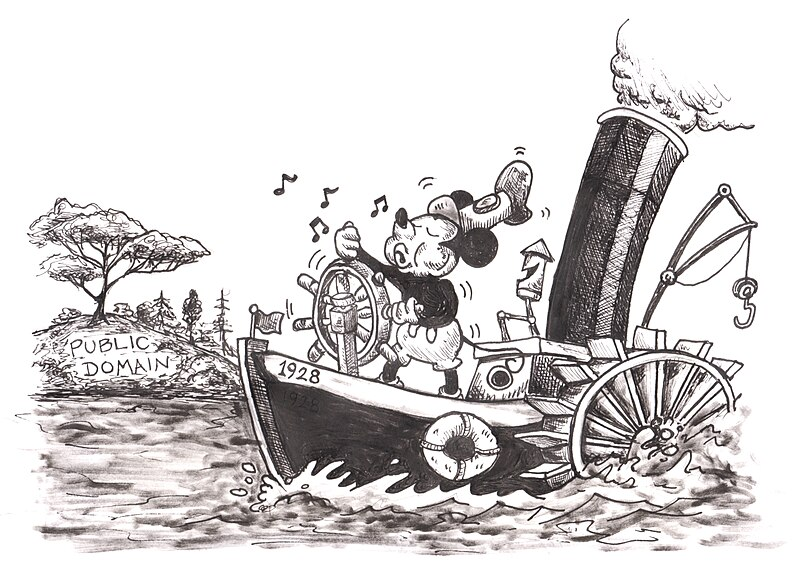
\includegraphics[width=.7\textwidth]{images/800px-Steamboat_Willie_Enters_the_Public_Domain.jpg}
\end{center}
         \hfill -- Doo Lee / CC BY 4.0 \\[-.5em]
         \hfill {\tiny \url{https://commons.wikimedia.org/wiki/File:Steamboat_Willie_Enters_the_Public_Domain.jpg}}

Yes. That mouse.


\end{frame}


\begin{frame}
\frametitle{FastPass System}

We're going to discuss the Disney FastPass and FastPass+ systems.

The full video: \url{https://www.youtube.com/watch?v=9yjZpBq1XBE}

It has a lot of Disney history, but let's try not to get distracted.

\end{frame}


\begin{frame}
\frametitle{Simulation Required}

Simulation is required because of the complexity here.

Some reasons why...

\end{frame}


\begin{frame}
\frametitle{Reasons for Complexity}

Every customer (requester) is an independent agent, which implies:
		\begin{itemize}
			\item They have different times of arrival at and departure from the park. Most arrive early in the day
			\item They have different preferences of what they want to do while there
			\item They have different willingness to wait for the things they want to do
			\item They may or may not be willing to come back another day
		\end{itemize}


\end{frame}


\begin{frame}
\frametitle{Reasons for Complexity}


The park has opening and closing times which implies:
		\begin{itemize}
		\item Requests cannot be submitted before opening time
		\item Requests cannot be submitted after closing time
		\item Requests submitted too close to closing time may not be served before closing
		\end{itemize}


\end{frame}


\begin{frame}
\frametitle{Reasons for Complexity}

\begin{itemize}
	\item The park has different services that each have their own service rate and any of them could be down for maintenance (indepedently of any others) \vspace{5em}
	\item The services have a fixed maximum capacity: you cannot make more seats on the rides or run them faster to get more people through quicker
\end{itemize}


\end{frame}


\begin{frame}
\frametitle{Relevance?}

Is this model relevant to software queueing?

Trip to Service Ontario should be arrive, get service, leave...\\
\quad And ideally not return for quite a while!

At the food hall I'll eventually get full...

\begin{center}
	\includegraphics[width=0.4\textwidth]{images/donuthell.jpg}
\end{center}

I go to the mouse park and want to do as much as I can do in the day.

\end{frame}


\begin{frame}
\frametitle{Relevant---Yes!}

Does it matter what the people ahead of me in the line do before or after?

Could we argue that after a ride a guest leaves and is replaced?

\end{frame}


\begin{frame}
\frametitle{User Types}

The simulation has many different user types. These determine:

\begin{enumerate}
	\item How long they stay
	\item When they balk
	\item What they want to do
\end{enumerate}

The third point covers preferences for rides and non-rides.


\end{frame}


\begin{frame}
\frametitle{Systems Three}

Our three systems:

\begin{enumerate}
	\item No Priority 
	\item FastPass
	\item FastPass+
\end{enumerate}

\begin{center}
	\includegraphics[width=0.5\textwidth]{images/fastpasslane.jpg}
\end{center}

Priority queues? Ratio of 4:1, 20:1, even 100:1.

\end{frame}


\begin{frame}
\frametitle{Try it Yourself}

Did you want to play around with the simulation yourself? 

\url{https://github.com/TouringPlans/shapeland}

It's Python, but it's not super complex.

\end{frame}

\begin{frame}
\frametitle{Nature of Results}

\begin{enumerate}
	\item Standby Waits
	\item Overall Waits
	\item Average Number of Rides Experienced
\end{enumerate}


\end{frame}


\begin{frame}
\frametitle{Standby Waits}

\begin{center}
	\includegraphics[width=\textwidth]{images/standbywait.png}
\end{center}

\end{frame}


\begin{frame}
\frametitle{Overall Waits}

\begin{center}
	\includegraphics[width=\textwidth]{images/overallwait.png}
\end{center}

\end{frame}


\begin{frame}
\frametitle{Rides Per Day}

\begin{center}
	\includegraphics[width=\textwidth]{images/ridesperday.png}
\end{center}

\end{frame}


\begin{frame}
\frametitle{Lessons and Limitations}

Priority passes don't affect wait times for most popular things...\\
\quad But do encourage more usage of less-popular things.

Is that improvement?

\begin{center}
	\includegraphics[width=0.4\textwidth]{images/mickey-think.jpg}
\end{center}


\end{frame}


\begin{frame}
\frametitle{Lessons and Limtations}
Simulation doesn't account for downtime during the day.

In the simple model of handling that, send people out of the queue.

More complex: what if people get a FastPass(+) as compensation?


\end{frame}


\begin{frame}
\frametitle{Inequality}

The knowledge factor results in huge inequality!

\begin{center}
	\includegraphics[width=0.4\textwidth]{images/halfthebattle.jpg}
\end{center}

Interesting lesson: complexity allows exploitation.

\end{frame}





\end{document}

